\section{Results: stiff regimes and speedup}
\label{sec:results}

\subsection{Lifted time-step limits}
Each level of the IMEX stack is verified to reproduce the explicit result at a matched
step before its lifted step is exercised (\cref{tab:cfl-lift}). Implicit viscosity is
stable to $50\times$ the explicit viscous CFL on Taylor--Green; the combined IMEX
reproduces the four-roll extensional blob $b_e^{xx}$ to $0.55\%$ at matched $\dt$ and
completes within ${\sim}2\%$ at $2$--$4\times$ the explicit viscous CFL where the
explicit scheme diverges; the linearly-implicit elastic stabilizer is consistent
($0.44\%$ vs.\ explicit at $0.1\times$ the elastic CFL) and remains stable at
$8\times$ the elastic CFL, where the explicit elastic force diverges; and the
semi-Lagrangian advection (\cref{sec:monolithic}) removes the final advective limit.
Crucially, the wall Helmholtz is solved by a DST-preconditioned CG that converges in a
handful of iterations independent of resolution ($17\!\to\!5$ at $N{=}128$), so the
lifted $\dt$ translates into a wall-clock gain rather than being consumed by the solve.

\begin{table}[t]\centering\small
\caption{Time-step limits lifted by each strategy (measured). ``reproduces'' is the
relative error against the explicit reference at matched $\dt$.}
\label{tab:cfl-lift}
\begin{tabular}{@{}llll@{}}
\toprule
strategy & lifts & max stable $\dt$ (vs explicit) & reproduces \\
\midrule
implicit viscosity & $\dx^2/\nu$ & $50\times$ (Taylor--Green) & 2nd-order retained \\
exact relaxation & $\dt\lesssim\tau$ & $\infty$ (step-strain exact) & machine precision \\
IMEX combined & both & $2$--$4\times$ (four-roll) & $0.55\%$ \\
elastic stabilizer & $\dx/c_s$ & $8\times$ (four-roll) & $0.44\%$ at $0.1\times$ \\
semi-Lagrangian adv. & $\dx/U$ & $6\times$ (soft disc) & $2.2\times10^{-3}$ at matched $\dt$ \\
\bottomrule
\end{tabular}
\end{table}

\begin{figure}[t]\centering
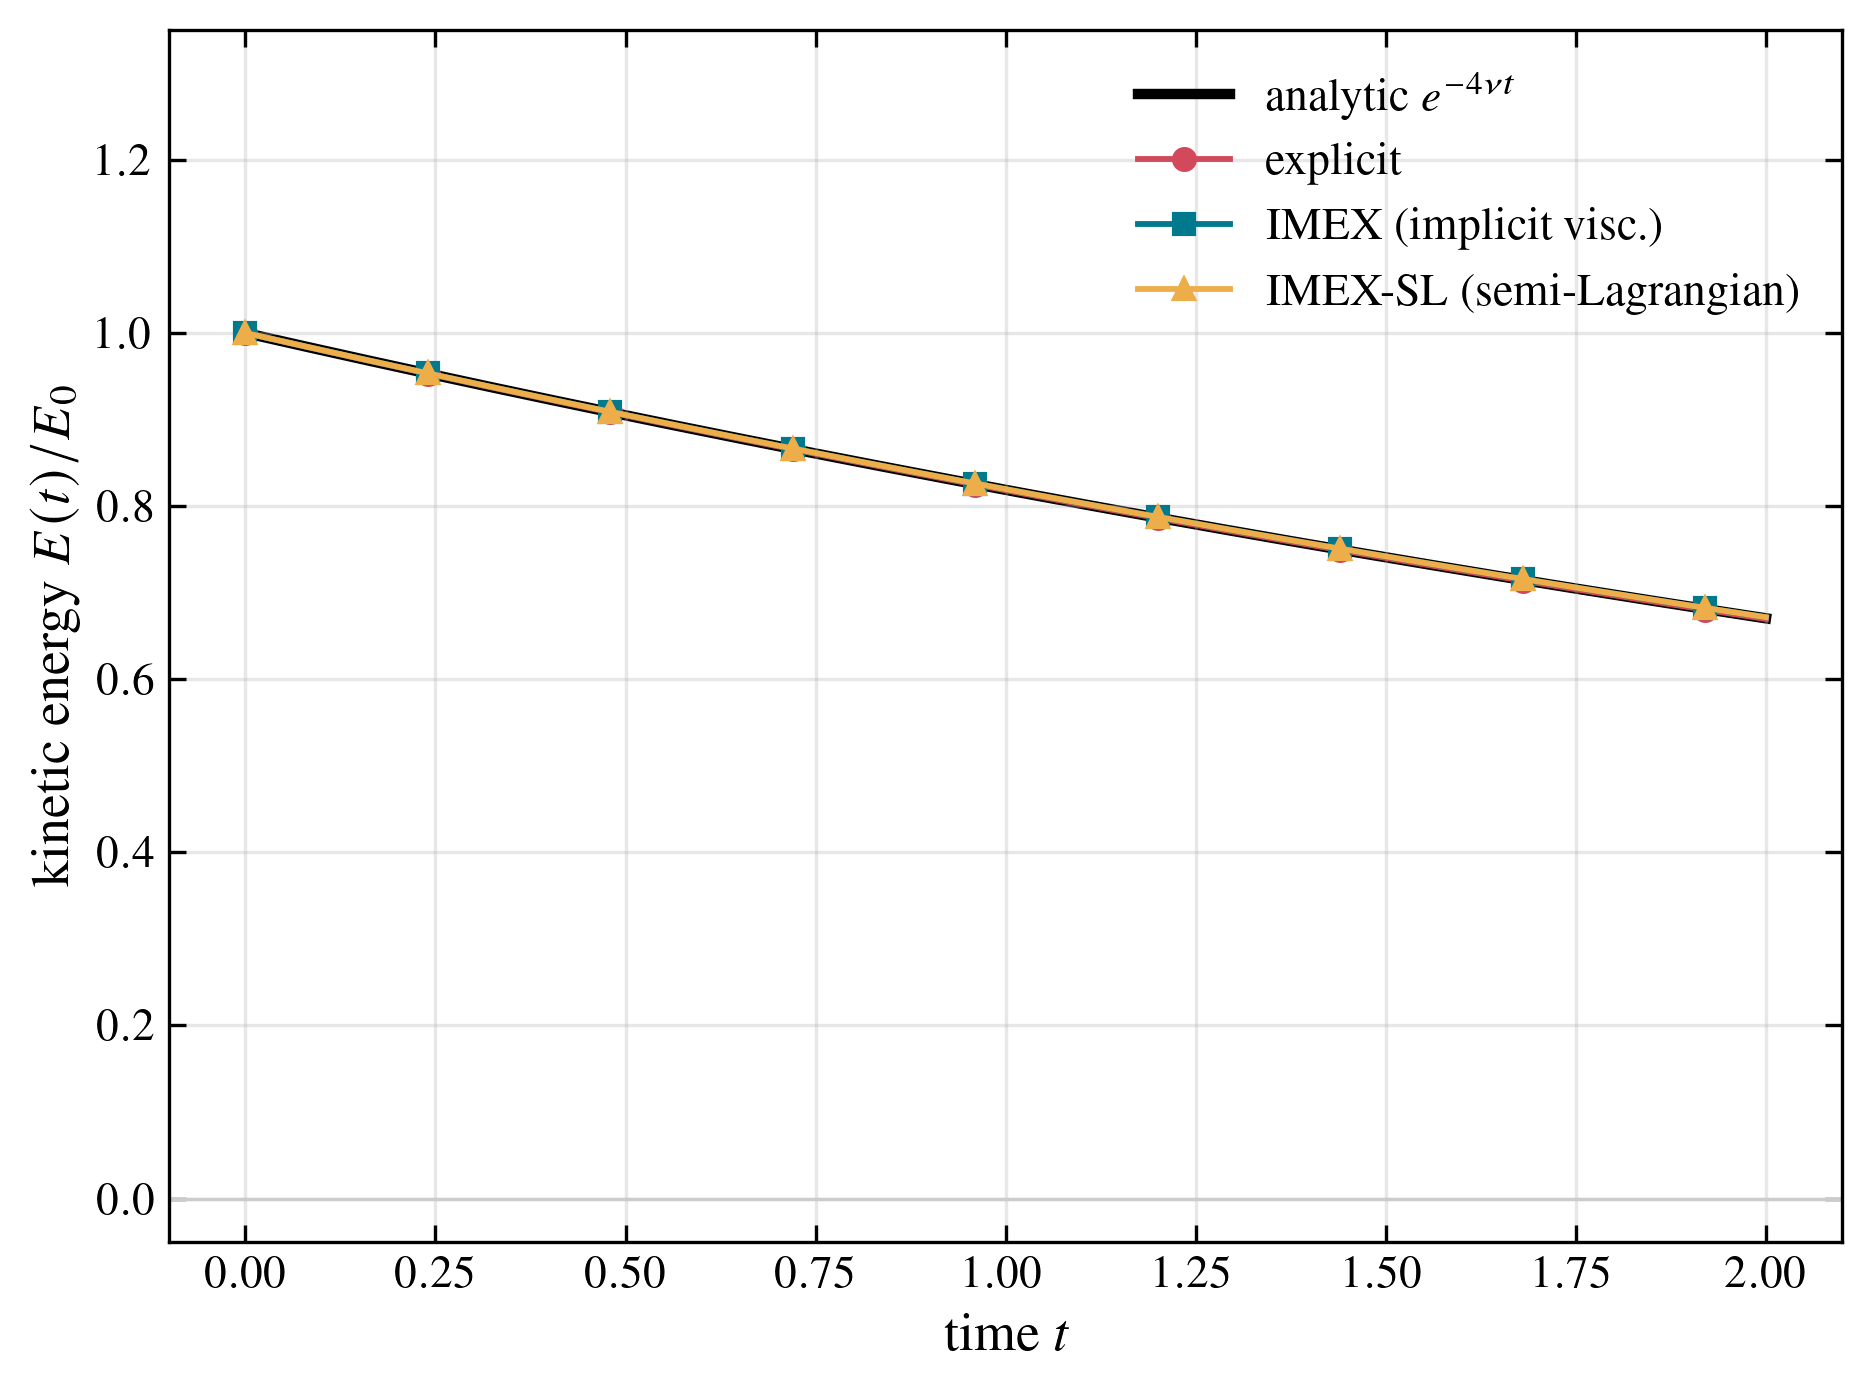
\includegraphics[width=0.66\linewidth]{figures/taylor_green_overlay.png}
\caption{Taylor--Green kinetic-energy decay: explicit, IMEX and IMEX-SL all track the
analytic $e^{-4\nu t}$ (here IMEX-SL uses central advection, so it coincides with IMEX).
The semi-Lagrangian branch is engaged only when the advective CFL is exceeded.}
\label{fig:tg-energy}
\end{figure}

\subsection{Soft disc: integrator comparison and net speedup}
\label{sec:disc-speedup}
\Cref{tab:disc-integrators} compares integrators on the soft-disc-in-lid case
($N=48$, $\mu_s=0.1$). The case is \emph{advection}-limited: implicit viscosity alone
(\texttt{imex}) reproduces the trajectory at the matched step ($\Delta$centroid
$2.2\times10^{-3}$) but cannot enlarge $\dt$, so it yields no speedup---confirming that
the last binding constraint is advection, not diffusion. Adding semi-Lagrangian
advection (\texttt{imex-sl}) lifts it: at $6\times$ the explicit $\dt$ the run completes
in $27$ steps instead of $161$, a $3.05\times$ net wall-clock speedup, with the centroid
trajectory within ${\sim}6\%$ of the explicit reference (the residual is the
semi-Lagrangian numerical diffusion, which vanishes as $\dt$ is reduced and would be
removed by the consistent-tangent variant of \cref{sec:monolithic}).

\begin{table}[t]\centering\small
\caption{Soft disc in lid-driven cavity ($N{=}48$), integrator comparison. Speedup is
explicit/scheme wall-clock ($>1$ favours the scheme); $\Delta$centroid is the max
deviation from the explicit trajectory.}
\label{tab:disc-integrators}
\begin{tabular}{@{}lllll@{}}
\toprule
integrator & $\dt$ (vs explicit) & steps & speedup & $\Delta$centroid \\
\midrule
explicit             & $1\times$ & $161$ & $1\times$      & --- \\
imex (implicit visc) & $1\times$ & $161$ & $0.97\times$   & $2.2\times10^{-3}$ \\
imex-sl              & $3\times$ & $54$  & $1.53\times$   & $5.6\times10^{-2}$ \\
imex-sl              & $6\times$ & $27$  & $\mathbf{3.05\times}$ & $6.0\times10^{-2}$ \\
\bottomrule
\end{tabular}
\end{table}

\paragraph{Work--precision and the regime where implicit pays off.}
\Cref{fig:work-precision} plots accuracy (max centroid deviation from a fine explicit
reference) against wall-clock time for the three FSI-applicable schemes at $N=64$ and
$N=128$. Two things are visible. At $N=64$ the semi-Lagrangian \texttt{imex-sl} scheme is
Pareto-optimal: taking $6$--$8\times$ the explicit step it reaches the same accuracy band in
$2.5$--$3.7\times$ less wall-clock, because it lifts the binding \emph{advective} limit at
essentially the explicit per-step cost. Implicit viscosity alone (\texttt{imex}) does
\emph{not} help here---advection, not diffusion, binds---and its iterative solve makes it
slower. At $N=128$, where the viscous limit binds the explicit step, the picture is
governed by the cost of the wall-bounded Helmholtz solve: the implicit step is
$\sim\!2\times$ larger but each step costs several times more, so implicit integration only
wins once the lifted-to-explicit step ratio exceeds that per-step overhead---the low-Reynolds,
stiff-solid, or finer-grid regime. The comparison thus \emph{delineates} rather than
universally asserts the benefit: the semi-Lagrangian step pays off broadly, while the
implicit viscous/elastic solves pay off specifically where the explicit step is throttled by
more than the solve cost.

\begin{figure}[t]\centering
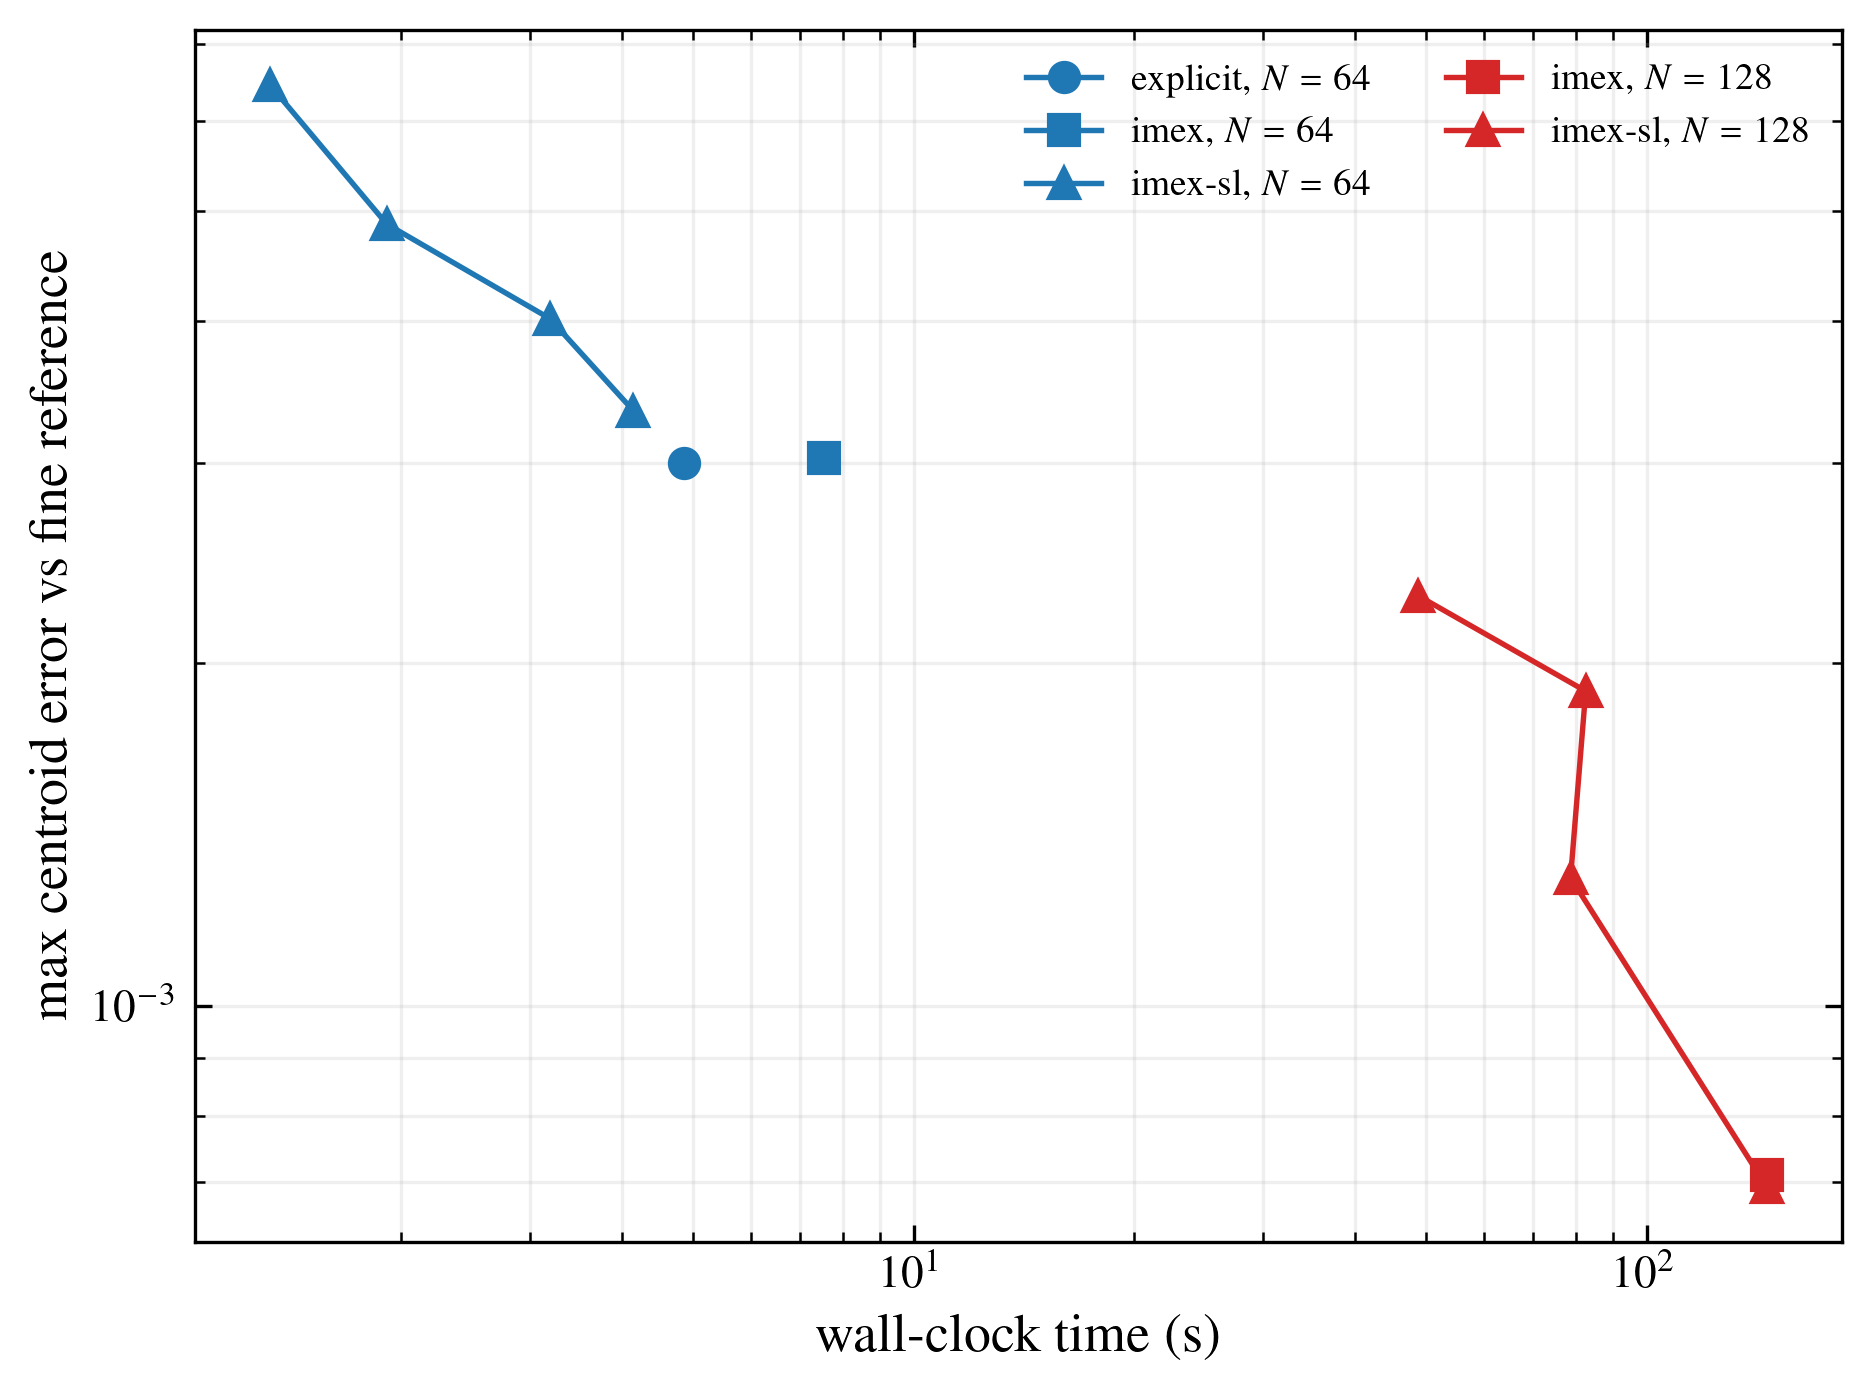
\includegraphics[width=0.68\linewidth]{figures/work_precision.png}
\caption{Work--precision on the soft-disc-in-lid FSI case: max centroid error vs.\
wall-clock for explicit, IMEX and IMEX-SL at $N=64$ (blue) and $N=128$ (red); IMEX-SL points
run at $2,4,6,8\times$ the explicit step. At $N=64$ IMEX-SL is Pareto-optimal (lower cost at
matched accuracy); at $N=128$ the wall-bounded implicit-solve cost per step offsets the
larger step, so the implicit advantage is regime-dependent.}
\label{fig:work-precision}
\end{figure}

\subsection{Semi-monolithic solver: accuracy and speedup}
\label{sec:results-mono}
The semi-monolithic scheme removes each explicit stability limit in turn
(\cref{tab:cfl-lift}): viscous ($\dx^2/\nu$, implicit Helmholtz), relaxation
($\dt\!\lesssim\!\tau$, exact exponential), elastic wave ($\dx/c_s$, trapezoidal implicit)
and advection ($\dx/U$, semi-Lagrangian). The trapezoidal elastic coupling is lossless on
the standing wave (\cref{sec:verification}: consistent-energy drift at round-off for every
$\dt$) where the stage-1 stabilizer damps the wave away; on the soft disc the combined
scheme delivers the $3.05\times$ net speedup of \cref{sec:disc-speedup}, the solve cost
staying low because the DST-preconditioned CG converges in ${\sim}5$--$7$ iterations
independent of $N$.

\paragraph{Semi-monolithic velocity--pressure (Newton--Krylov).} Making advection
implicit \emph{and consistent}---rather than semi-Lagrangian---removes the split/SL error
entirely. The semi-monolithic scheme (\cref{alg:mono}) solves the coupled $(\uv,p)$ system
by JFNK, preconditioned by one IMEX step and the projection. On Taylor--Green it reproduces
the analytic decay ($1.5\times10^{-4}$ at $\dt$ below the CFL) and, crucially, stays
\emph{accurate} far above the advective CFL: at $5\times$ the CFL its error is
$1.1\times10^{-3}$ (clean $O(\dt)$), versus the $2.7\times10^{-2}$ diffusion floor of the
semi-Lagrangian scheme at the same step---an order of magnitude more accurate at large
$\dt$, with Newton converging in ${\sim}3$ iterations per step. This is the accuracy
advantage of the monolithic route; extending it to the fully-coupled solid
(\cref{sec:monolithic}) is future work.
